\section{Contexto y alcance}

%La integración continua, o CI, como se conoce a menudo por su abreviatura en inglés, es una práctica de desarrollo de software mediante la cual los desarrolladores combinan los cambios de código en un repositorio central de forma periódica, comprobándose que el código se comporta de la forma esperada a través de pruebas automáticas. 
%Es decir, CI como proceso significa que cada cambio subido a un sistema de control de versiones ha sido puesto a prueba, validado y aceptado.

%\cotutor{Dentro de la definición de CI, debe haber una referencia al enfoque DevOps, siendo el IC un aparte fundamental de este enfoque, promoviendo la automatización la colaboración entre desarrolladores y obtención de feedback constante}

%\cotutor{Introduces el despliegue del software, pero esto vá un poco más allá del CI y pasa a ser CI/CD. Es cierto que lo que denominamos sistemas o herramientas de CI se ocupan también de estos procesos. Te dejo a continuación una imagen que ilustra bastante bien esto. En Integración Continua buscamos integrar el código constantemente, para lo cual nos ayudamos de scripts automáticos para compilar y ejecutar los test de la nueva versión. En ciertos casos, nos interesa hacer entrega continua, es decir, entregar un software, que podría ser una libreria o una aplicación final en forma de artefactos. En este caso, nos interesa que el software se entregue en una forma continua, es decir, que se entregue una vez que se haya compilado y se haya probado, siendo la continuación directa de los pasos seguidos en CI. Por último, se podría automatizar también el proceso de despliegue (típico de aplicaciones web).}

La integración, entrega y despliegue continuo, o CI/CD, como se conoce a menudo por su abreviatura en inglés, es un método que va a permitir distribuir aplicaciones a clientes de forma frecuente gracias a la automatización en las etapas del desarrollo. Para los equipos de desarrollo y de operaciones es solución a los diferentes problemas que pueda generar la integración del código nuevo.

En concreto, en el proceso de integración y distribución continua existen un conjunto de prácticas conocidas con el nombre de ``canales de CI/CD'' encargadas de la automatización y la supervisión permanente en todo el ciclo de vida de las aplicaciones, teniendo en cuenta etapas como la implementación, pruebas, integración y/o distribución. Estas prácticas cuentan con el respaldo de los equipos de desarrollo y de operaciones, los cuales trabajan en conjunto de manera ágil con un enfoque SRE (ingeniería de confiabilidad del sitio) o de DevOps \cite{redHatCICD}.

La integración continua, o ``CI'', se trata de un proceso de automatización para los desarrolladores y su éxito supone que se diseñen, prueben y combinen los cambios nuevos en el código de una aplicación con regularidad en un repositorio compartido.

La entrega y/o despliegue continuo, o ``CD'', son conceptos referidos a la automatización de las etapas posteriores del proceso. Por lo general, la entrega continua se refiere a que los cambios que implementan los desarrolladores en una aplicación se someten a pruebas automáticas de errores y se cargan en un repositorio de almacenamiento de código como por ejemplo GitHub y el despliegue continuo hace referencia al lanzamiento automático de los cambios que implementan dichos desarrolladores desde el repositorio de código hasta el entorno de producción, en el que estarán a disposición del usuario final.

%Anteriormente, era común que los desarrolladores de un equipo trabajasen aislados durante un largo periodo de tiempo y solo intentasen combinar los cambios en la versión final una vez completado el trabajo. Como consecuencia, la combinación de los cambios en el código resultaba ser una ardua tarea, dando lugar a que fuese más difícil proporcionar las actualizaciones a los clientes con rapidez.

%Con la integración continua, los desarrolladores pueden enviar estos cambios de código de forma periódica a un repositorio compartido con un sistema de control de versiones como Git, y antes de cada envío, los desarrolladores pueden elegir ejecutar una serie de pruebas unitarias sobre el código como medida de verificación adicional antes de la integración.

Por lo tanto, los objetivos principales de la integración continua consisten en detectar y arreglar errores con mayor rapidez, mejorar la calidad del software y reducir el tiempo que se tarda en validar y publicar nuevas actualizaciones del código fuente.

\begin{figure}[h]
    \centering
    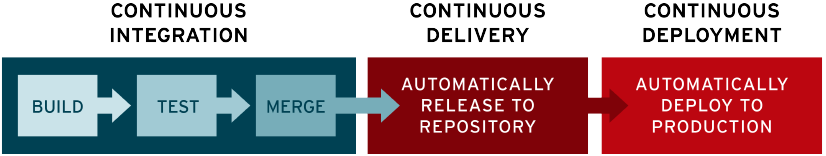
\includegraphics[width=0.75\textwidth,clip=true]{imgs/ci-cd-flow-desktop.png}
    \caption{Diagrama de CI/CD}
\end{figure}

Esta trabajo pondrá más énfasis en lo que a la parte de ``CI'' se refiere y en aras de comprender lo que engloba cabría definir también conceptos como ``build'' o escenario CI: un ``build'' es mucho más que una compilación, también engloba el proceso de pruebas, inspección de código y despliegue del mismo, a parte de otras cosas. Actúa como el proceso para juntar el código fuente y verificar que el software funcione como una unidad cohesiva. Un escenario de CI comienza cuando el desarrollador envía el código fuente al repositorio. En un proyecto típico, {personas} con diferentes roles pueden realizar cambios que desencadenan un ciclo de CI: los desarrolladores cambian el código fuente, los administradores de bases de datos (DBA) cambian las definiciones de las tablas, los equipos de desarrollo e implementación cambian los archivos de configuración, los equipos de interfaz cambian las especificaciones DTD/XSD y más.

Los pasos en un escenario de CI típicamente serán más o menos de la siguiente forma \cite{CI_Paul_Duvall}:
\begin{enumerate}
    \item El desarrollador envía código al repositorio de código, gestionado con un sistema de control de versiones. 
    Mientras tanto, el servidor de CI en la máquina de compilación de integración sondea este repositorio en busca de cambios (cada pocos minutos, por ejemplo).
    \item Poco después de que se produzca una confirmación, el servidor de CI detecta que se han producido cambios en el repositorio de control de versiones, dando lugar a que se recupere la última copia del código del repositorio y ejecute un script de compilación. Dicho script de compilación se encarga de ejecutar los tests y comprobar que el software se puede construir.
    \item El servidor de CI captura los resultados de la compilación y ejecución de los test, enviándolos, por ejemplo, por correo electrónico a los miembros del equipo.
\end{enumerate}

\begin{figure}[h]
    \centering
    \includegraphics[width=0.75\textwidth,clip=true]{\ciDiagram}
    \caption{Diagrama de CI}
\end{figure}

\section{Enfoque DevOps}
DevOps es un marco de trabajo que describe los enfoques para agilizar los procesos con los que una idea, como pudiera ser una nueva funcionalidad de software por ejemplo, pasa del desarrollo a la implementación, en un entorno de producción. Es decir, el enfoque DevOps va impulsar un mejor desarrollo de aplicaciones en menos tiempo con el objetivo de lograr la satisfacción del cliente prestando sus servicios eficazmente.

Para el correcto funcionamiento de la filosofía DevOps, se requiere que los equipos de desarrollo y operaciones se comuniquen con frecuencia y aborden su trabajo con empatía hacia sus compañeros de equipo. Por ello con DevOps se fomenta una comunicación continua más fluida, la colaboración y la transparencia entre equipos de desarrollo de aplicaciones y sus equivalentes en operaciones tecnológicas.

DevOps también se ha creado para impulsar la innovación empresarial ya que propicia que cada empresa se ponga como objetivo ofrecer un mejor servicio cada vez, en menos tiempo, de mejor calidad y con mayor seguridad a sus clientes finales; por ejemplo, incrementando la frecuencia de versiones de producto.

\subsection{Proceso de DevOps}
Para muchos de los equipos que utilizan metodologías ágiles para el desarrollo de software, el enfoque DevOps no es algo secundario. De hecho, el primero de los 12 principios del Manifiesto Ágil es el siguiente: ``Satisfacer a los clientes mediante la distribución de software continua y oportuna'' y es por ello por lo que la metodología de integración, entrega y despliegue continuo (CI/CD) es tan importante para los equipos de DevOps.

Según un estudio de ``International Data Corporation'' (IDC), el 85 \% de los líderes de TI afirman que la automatización es primordial para su estrategia de DevOps, debido a que la automatización permite que las infraestructuras admitan cambios de código constantes acompañando al enfoque DevOps. Además, permite que los entornos se expandan con facilidad y de manera constante \cite{redHatDevOps}. Gracias a que la automatización se ocupa de tareas tediosas y repetitivas, el personal más capacitado puede dedicarse a actividades de mayor importancia.

\subsection{Métodos de DevOps}
A continuación se definen varios métodos de DevOps que las organizaciones utilizan habitualmente para acelerar y mejorar el desarrollo de su producto:
\begin{compactitem}
    \item \textbf{\underline{Scrum}}: define cómo los miembros de un equipo deben cooperar para conseguir acelerar los proyectos de desarrollo y control de calidad.
    \item \textbf{\underline{Kanban}}: mediante un tablero compuesto, generalmente, por tres columnas: “Por hacer”, “En proceso” y “Hecho” se demuestra dónde están los cuellos de botella en el proceso y qué es lo que impide que el flujo de trabajo sea ininterrumpido.
    \item \textbf{\underline{Agile}}: se refiere a un grupo de metodologías de desarrollo de software basadas en el desarrollo iterativo, donde los requisitos y las soluciones evolucionan a través de la colaboración entre equipos multifuncionales y autoorganizados.
\end{compactitem}

%\subsection{Cadena de herramientas}
%A continuación se ofrece un ejemplo de herramientas que se emplean en las diversas etapas del ciclo de DevOps:
%\begin{compactitem}
    %\item \textbf{\underline{Planificación}}: fase en la que se definen los requisitos y valores empresariales. Algunas herramientas relativas a esta fase serían: Jira o Git.
    %\item \textbf{\underline{Codificación}}: implica el diseño del software y la creación del código. Algunas herramientas relativas a esta fase serían: GitHub, GitLab, Bitbucket o Stash.
    %\item \textbf{\underline{Compilación}}: fase en la que se gestionan las versiones y las compilaciones del software, y se utilizan herramientas automatizadas que ayudan a compilar y crear paquetes de código para publicarlos después en producción. Algunas herramientas relativas a esta fase serían: Docker, Ansible, Puppet, Chef, Gradle, Maven o JFrog Artifactory.
    %\item \textbf{\underline{Prueba}}: incluye la realización de pruebas continuas (manuales o automatizadas). Algunas herramientas relativas a esta fase serían: JUnit, Codeception, Selenium, Vagrant, TestNG o BlazeMeter.
    %\item \textbf{\underline{Puesta en marcha}}: fase en la que se emplean herramientas que ayudan a gestionar, coordinar, programar y automatizar las tareas de producción de las versiones de productos. Algunas herramientas relativas a esta fase serían: Puppet, Chef, Ansible, Jenkins, Kubernetes, OpenShift, OpenStack, Docker o Jira.
    %\item \textbf{\underline{Funcionamiento}}: fase en la que se gestiona el software durante su producción. Algunas herramientas relativas a esta fase serían: Ansible, Puppet, PowerShell, Chef, Salt o Otter.
    %\item \textbf{\underline{Supervisión}}: se identifica y recopila información sobre problemas que surgen en una versión de software específica. Algunas herramientas relativas a esta fase serían: New Relic, Datadog, Grafana, Wireshark, Splunk, Nagios o Slack.
%\end{compactitem}

\subsection{Prácticas de DevOps}
Las prácticas de DevOps son un reflejo de la idea de automatización y mejora continuas e incluyen lo siguiente \cite{netAppDevOps}:
\begin{compactitem}
    \item Desarrollo continuo.
    \item Realización de pruebas continuas.
    \item \textbf{\underline{Integración continua (CI)}}.%: se combinan herramientas de gestión de configuración (CM) con otras herramientas de pruebas y desarrollo para saber qué cantidad del código que se está creando está listo para pasar a producción. Para ello, debe existir un intercambio fluido de información entre las fases de prueba y de desarrollo que permita identificar y resolver con rapidez problemas en el código.
    \item Entrega y despliegue continuo (CD).
    \item Supervisión continua.
    \item Infraestructura como código.
\end{compactitem}

%\subsection{Ventajas}
%A continuación se enumeran las ventajas que DevOps ofrece:
%\begin{compactitem}
    %\item Una mejor y más rápida entrega de productos.
    %\item Resolución de problemas en menos tiempo y con menor complejidad.
    %\item Mejor escalabilidad y disponibilidad.
    %\item Entornos de funcionamiento más estables.
    %\item Mejor utilización de los recursos.
    %\item Mayor automatización.
    %\item Mayor visibilidad de resultados del sistema.
    %\item Mayor innovación.
%\end{compactitem}

\section{Prerrequisitos de la integración continua}
Existen cuatro componentes requeridos para llevar a cabo el proceso de integración continua.
\begin{compactitem}
    \item Tener conexión a un sistema de control de versiones como por ejemplo git o subversion ``svn''.
    \item Tener un script de compilación ``build'' con el que construir y ejecutar los test del software desarrollado.
    \item Tener un mecanismo de retroalimentación, como el envío de correos electrónicos.
    \item Tener un proceso para integrar los cambios del código fuente (de forma manual o mediante un servidor de integración continua).
\end{compactitem}

\section{Subprocesos de la integración continua}
Mediante la integración continua y automática de bases de datos, pruebas, inspección de código, despliegue y ``feedback'' o retroalimentación, permite al sistema de CI reducir riesgos comunes del software generando una mayor confianza y comunicación sobre los diferentes cambios que se vayan a realizar y los errores que se puedan provocar con la incorporación de dichos cambios. 

Una vez que se ejecuta una compilación o ``build'' automatizada con cada cambio en el sistema de control de versiones, se pueden agregar otras funciones o subprocesos al sistema de CI. Algunas funciones dependen de otras; por ejemplo, las pruebas automatizadas dependen de la compilación del código fuente. Este proceso repetitivo puede ayudar a reducir riesgos a lo largo del ciclo de vida del desarrollo.

Estos subprocesos quedarían definidos de la siguiente forma:
\begin{compactitem}
    \item \textbf{Compilación del código fuente}. Implica la creación de un código ejecutable a partir de fuentes legibles.
    \item \textbf{Integración de base de datos}, siendo la base de datos una parte integral de las aplicaciones software.
    \item \textbf{Ejecución de pruebas o “testing”}. Son una parte fundamental de la integración continua. Sin pruebas automatizadas, es difícil para los desarrolladores u otras partes interesadas del proyecto tener confianza en los cambios de software.
    \item \textbf{Inspección de código}. Proceso utilizado para mejorar la calidad del software al hacer cumplir ciertas reglas.
    \item \textbf{Despliegue}. Siendo una parte más enfocada en la parte de CD.
    \item \textbf{Documentación y “feedback”}. Una característica fundamental de los buenos sistemas de CI es la velocidad, y su esencia es proporcionar retroalimentación oportuna a los desarrolladores y partes interesadas del proyecto.
\end{compactitem}

%A continuación se describen más en detalle estos subprocesos.

%\subsection{Compilación del código fuente}
%La compilación continua de código fuente es una de las características más básicas y comunes de un sistema CI. De hecho, es tan común que casi se ha convertido en sinónimo de CI. La compilación implica la creación de un código ejecutable a partir de fuentes legibles. Sin embargo, CI es mucho más que compilación de código fuente.

%\subsection{Integración de base de datos}
%Hay personas que consideran la integración del código fuente y la integración de bases de datos como procesos completamente separados, siempre llevados a cabo por diferentes grupos. Esto es porque la base de datos es una parte integral de las aplicaciones software. 

%Utilizando un sistema de integración continua se puede garantizar la integración de una base de datos a través de una única fuente: el repositorio de control de versiones. Para habilitar la integración continua de bases de datos en el proceso de construcción de un sistema de CI, tratamos el código fuente de la base de datos, las secuencias de comandos del ``Lenguaje de Definición de Datos'' (DDL), las secuencias de comandos del ``Lenguaje de Manipulación de Datos'' (DML), las definiciones de procedimientos almacenados, las particiones, etc. de la misma manera que cualquier otro código fuente del sistema. Por ejemplo, cuando un miembro del proyecto modifica un script de base de datos y lo confirma en el sistema de control de versiones, el mismo script de compilación que integra el código fuente reconstruirá la base de datos y los datos como parte del proceso de compilación.

%\subsection{Ejecución de pruebas o “testing”}
%Se considera que la integración continua sin pruebas automatizadas no sería integración continua. Sin pruebas automatizadas, es difícil para los desarrolladores u otras partes interesadas del proyecto tener confianza en los cambios de software. La mayoría de los desarrolladores de proyectos que utilizan un sistema de CI usan herramientas de prueba unitaria como JUnit para ejecutar pruebas. Además, se pueden ejecutar diferentes categorías de pruebas desde un sistema de CI con el objetivo de acelerar el proceso de compilación. Estas categorías pueden incluir de unidad, componente, sistema, carga/rendimiento, seguridad y otros.

%\subsection{Inspección de código}
%Las inspecciones de código automatizadas se utilizan para mejorar la calidad del software al hacer cumplir ciertas reglas. Por ejemplo, un proyecto puede tener una regla de que ninguna clase puede tener más de 300 líneas de código sin comentarios. Utilizando un sistema de CI se pueden ejecutar estas reglas automáticamente contra una base de código.

%\subsection{Despliegue}
%El despliegue continuo permite entregar software funcional e implementable en cualquier momento. Esto significa que un propósito clave de un sistema de CI es generar los paquetes de artefactos software con los últimos cambios de código y ponerlos a disposición de un entorno de prueba. 

%Entre otras cosas, se deben realizar las siguientes acciones en un proceso de despliegue:
%\begin{compactitem}
    %\item verificar los archivos fuente del repositorio de control de versiones, 
    %\item realizar la compilación de los mismos, 
    %\item todas las pruebas e inspecciones del código se deben ejecutar con éxito,
    %\item etiquetar la versión
    %\item y preparar los archivos de implementación.
%\end{compactitem}

%Además, una buena práctica consiste en incluir la capacidad de revertir automáticamente todos los cambios aplicados en el despliegue.

%\subsection{Documentación y “feedback”}
%Muchos desarrolladores trabajan bajo la firme creencia de que la documentación pertenece al código fuente, de hecho, ese código claro y conciso con nombres de métodos, variables y clases bien elegidos es la mejor documentación. No obstante, un sistema CI también puede proporcionar bastantes beneficios en lo que a la documentación se refiere. Una característica fundamental de los buenos sistemas de CI es la velocidad, y su esencia es proporcionar retroalimentación oportuna a los desarrolladores y partes interesadas del proyecto. Para generar documentación se pueden utilizar herramientas como Maven, Javadoc o NDoc y, además, existen otras herramientas que pueden generar diagramas de clase y e información relevante, todo basado en el código fuente subido o “committed” al repositorio de control de versiones.

\section{Valor de la integración continua}
A alto nivel, el valor u objetivos de la integración continua serían:
\begin{enumerate}
    \item Reducir riesgos.
    \item Reducir procesos manuales repetitivos.
    \item Generar software desplegable en cualquier momento y en cualquier lugar.
    \item Habilitar una mejor visibilidad del proyecto.
    \item Establecer una mayor confianza en el producto software del equipo de desarrollo.
\end{enumerate}
\subsection{Reducir riesgos}
Integrando muchas veces al día se pueden reducir los riesgos de un proyecto software. Llevarlo a cabo facilita la detección de defectos, la medición del estado del software y la reducción de suposiciones.
\begin{compactitem}
    \item Los defectos se detectan y se solucionan antes: debido a que CI integra y ejecuta pruebas e inspecciones varias veces al día, existe una mayor probabilidad de que los defectos se descubran en el momento en el que son introducidos en el proyecto (es decir, cuando el código se registra en el repositorio de control de versiones) en lugar de durante las pruebas de último ciclo.
    \item El estado del software se puede medir: al incorporar pruebas e inspecciones continuas en el proceso de integración automatizado, los atributos de estado del producto de software (como la complejidad por ejemplo) se pueden rastrear a lo largo del tiempo.
    \item Reduce las suposiciones: al reconstruir y probar el software en un entorno limpio utilizando el mismo proceso y los mismos scripts de forma continua, se pueden reducir las suposiciones (ya sean porque se estuviesen contabilizando librerías de terceros o que se estuviesen utilizando variables de entorno, por ejemplo).
\end{compactitem}
La integración continua proporciona una red de seguridad para reducir el riesgo de que se introduzcan defectos en el código fuente. Los siguientes son algunos de los riesgos que CI ayuda a mitigar:
\begin{compactitem}
    \item Falta de software cohesivo e implementable.
    \item Descubrimiento tardío de defectos.
    \item Software de baja calidad.
    \item Falta de visibilidad del proyecto.
\end{compactitem}
\subsection{Reducir procesos repetitivos}
los procesos repetitivos pueden ocurrir en todas las actividades del proyecto, incluida la compilación de código, la integración de la base de datos, las pruebas, la inspección del código fuente, el despliegue y la retroalimentación o “feedback” y reducirlos supone un ahorro en tiempo, coste y esfuerzo. Al utilizar integración continua se aumenta la capacidad de garantizar los siguientes aspectos:
\begin{compactitem}
    \item El proceso se ejecuta de la misma manera cada vez.
    \item Se sigue un proceso ordenado.
    \item Los procesos se ejecutarán cada vez que se produzca una confirmación en el repositorio de control de versiones. 
    \item La reducción del trabajo en procesos repetitivos libera a las personas para que realicen trabajo de mayor valor.
    \item La capacidad de superar la resistencia (de otros miembros) para implementar mejoras mediante el uso de mecanismos automatizados para procesos importantes como las pruebas.
\end{compactitem}
\subsection{Generar software desplegable}
CI permite lanzar software desplegable en cualquier momento de tiempo, y desde una perspectiva externa, este es el beneficio más obvio de la integración continua. Se podría hablar indefinidamente sobre la mejora de la calidad del software y la reducción de los riesgos, pero el software desplegable es el activo más tangible para aquellas personas que no estén tan habituadas a ver e interpretar código fuente, como clientes o usuarios.
\subsection{Habilitar una mejor visibilidad del proyecto}
CI proporciona la capacidad de notar tendencias y tomar decisiones efectivas, ayudando a la hora de poder innovar en nuevas mejoras. Los proyectos software sufren cuando no hay datos reales o recientes para respaldar las decisiones que se toman, dando lugar a que todos ofrezcan sus mejores conjeturas. Por lo general, los miembros de un proyecto recopilan esta información manualmente, lo que supone mucho esfuerzo y que, a menudo, la información nunca se recopile. 

CI tiene los siguientes efectos positivos:
\begin{compactitem}
    \item Decisiones eficaces: un sistema de CI puede proporcionar información justo a tiempo sobre el estado de construcción reciente y las métricas de calidad. Algunos sistemas de CI también pueden mostrar tasas de defectos y estados de finalización de características.
    \item Notar tendencias: dado que la integración de proyectos ocurre con frecuencia con un sistema de CI, la capacidad de notar tendencias en el éxito o el fracaso de la construcción, la calidad general u otra información pertinente del proyecto se vuelve posible.
\end{compactitem}
\subsection{Establecer una mayor confianza en el producto}
En general, la aplicación eficaz de las prácticas de CI puede proporcionar una mayor confianza en la producción de un producto de software. Con cada compilación, el equipo de desarrollo es consciente de que se ejecutan pruebas contra el software para verificar el comportamiento, que se cumplen los estándares de codificación y diseño del proyecto. El hecho de que un sistema de CI pueda informar de si algo sale mal implica que los desarrolladores y otros miembros del equipo tengan más confianza a la hora de poder realizar cambios.

\section{Herramientas de integración continua}
Actualmente existen una gran cantidad de herramientas de integración continua, a comentar, por su grado de relevancia y uso, las siguientes:

- \textbf{\underline{Jenkins}}: es un sistema de integración continua de código abierto y autónomo que se utiliza para mecanizar todo tipo de trabajos asociados a la creación, prueba y entrega o despliegue de productos software.\\
Se puede instalar de tres formas distintas: con paquetes del sistema nativo, a través de la plataforma de gestión de contenedores Docker o incluso de forma independiente en cualquier máquina que tenga instalado un JRE (Java Runtime Environment).
\begin{figure}[h]
    \centering
    \includegraphics[width=0.25\textwidth,clip=true]{\logoJenkins}
    \caption{Logo de Jenkins.}
\end{figure}

- \textbf{\underline{Travis CI}}: escrito en Ruby, es un servicio de integración continua utilizado para crear y probar proyectos de software alojados en las siguientes plataformas de hospedaje de código fuente: GitHub, GitLab, Bitbucket o Assembla. Fue el primer servicio de CI que permitió realizar el proceso de integración continua a proyectos de código abierto de forma gratuita.

Algunas de las características y funciones que proporciona Travis CI son:
\begin{compactitem}
    \item Configuración rápida.
    \item Vistas de construcción en tiempo real.
    \item Sistemas de base de datos preinstalados.
    \item Limpieza de máquinas virtuales en cada compilación.
    \item Compatibilidad con Linux, Mac e iOS.
\end{compactitem}

\begin{figure}[h]
    \centering
    \includegraphics[width=0.25\textwidth,clip=true]{\logoTravis}
    \caption{Logo de Travis.}
\end{figure}

- \textbf{\underline{Circle CI}}: es un servicio de integración caracterizado por los aspectos comentados a continuación:
\begin{compactitem}
    \item Flujos de trabajo para la mecanización de tareas.
    \item Compatible con Docker.
    \item CPU y RAM configurables con el objetivo de adaptar dichos flujos de trabajo al equipo.
    \item Soporte independiente del lenguaje de programación: acepta cualquier lenguaje de programación desarrollado en Windows, Linux o macOS.
    \item Información almacenable en memoria caché.
    \item Ejecución de compilaciones locales mediante SSH para una depuración trivial.
    \item Seguridad: LDAP para gestión de usuarios, aislamiento de máquinas virtuales de forma completa, etc.
    \item Monitorización del estado y optimización de flujos de trabajo de forma sencilla.
\end{compactitem}
Además, cuenta con dos opciones de hospedaje: en la nube o en servidor y con tres opciones de precios: ``Free'' 0 dólares al mes, ``Performance'' 30 dólares al mes y ``Scale'' con un precio a medida.
\begin{figure}[h]
    \centering
    \includegraphics[width=0.25\textwidth,clip=true]{\logoCircleCI}
    \caption{Logo de Circle CI.}
\end{figure}

- \textbf{\underline{GitLab CI}}: es la parte de GitLab que se encarga de la integración continua, entrega y/o despliegue continuo. Con GitLab CI/CD se puede probar, crear y publicar software sin necesidad de tener que utilizar una aplicación de terceros.
\begin{figure}[h]
    \centering
    \includegraphics[width=0.125\textwidth,clip=true]{\logoGitLabCI}
    \caption{Logo de GitLab CI.}
\end{figure}

- \textbf{\underline{GitHub Actions}}: las acciones de GitHub automatizan tareas dentro del ciclo de vida de un desarrollo software. Ejecutan comandos después de que se haya producido algún evento específico.

\begin{figure}[h]
    \centering
    \includegraphics[width=0.375\textwidth,clip=true]{\logoGitHubActions}
    \caption{Logo de GitHub Actions.}
\end{figure}

El siguiente diagrama muestra cómo se pueden usar las acciones de GitHub para ejecutar automáticamente scripts de prueba de software: un evento activa automáticamente un “flujo de trabajo”, que contiene un trabajo. Luego, dicho trabajo usa pasos para controlar el orden en el que se ejecutan las acciones. %Estas acciones son los comandos que automatizan las pruebas de software. Además, hay múltiples componentes de GitHub Actions que trabajan juntos para ejecutar trabajos.
\begin{figure}[h]
    \centering
    \includegraphics[width=0.4\textwidth,clip=true]{\githubActionsDiagram}
    \caption{Flujo de trabajo de GitHub Actions.}
\end{figure}

%- \textbf{\underline{Azure pipelines}}: compila y prueba automáticamente proyectos de código para que estén disponibles para otros usuarios. Funciona con prácticamente cualquier tipo de proyecto o lenguaje.

%\begin{figure}[h]
    %\centering
    %\includegraphics[width=0.4\textwidth,clip=true]{\logoAzurePipelines}
    %\caption{Logo de Azure Pipelines.}
%\end{figure}

%Sus principales características son:
%\begin{compactitem}
    %\item Multilenguaje y multiplataforma: permite compilar, probar e implementar aplicaciones de Node.js, Python, Java, PHP, Ruby, C/C++, .NET, iOS y Android. Además, permite ejecutar archivos en paralelo en Linux, macOS y Windows.
    %\item Compatible con contenedores y Kubernetes: permite compilar e insertar fácilmente imágenes en registros de contenedor, como Docker Hub y Azure Container Registry. Además, permite implementar contenedores en hosts individuales o en Kubernetes.
    %\item Extensible: permite explorar e implementar una gran variedad de tareas de compilación, pruebas e implementación creadas por la comunidad, junto con cientos de extensiones, desde Slack hasta SonarCloud.
    %\item Soluciones en cualquier nube: disponible la entrega continua (CD) del software en cualquier nube como Azure, AWS y GCP.
    %\item Gratis para código abierto: asegura canalizaciones rápidas de integración y entrega continuas (CI/CD) para proyectos de código abierto.
    %\item Características y flujos de trabajo avanzados: compatibilidad con YAML, integración de pruebas, validación de versiones, informes, etc.
%\end{compactitem}

%- \textbf{\underline{Bamboo}}: Atlassian Bamboo es un servidor de integración continua (CI) e implementación que ayuda a los equipos de desarrollo de software proporcionando:
%\begin{compactitem}
    %\item creación y pruebas automatizadas del estado del código fuente del software.
    %\item actualizaciones en compilaciones correctas y fallidas.
    %\item herramientas de presentación de informes para el análisis estadístico.
%\end{compactitem}

%\begin{figure}[h]
    %\centering
    %\includegraphics[width=0.3\textwidth,clip=true]{\logoBamboo}
    %\caption{Logo de Bamboo.}
%\end{figure}

%- \textbf{\underline{Codeship}}: CloudBees CodeShip es una solución de software como servicio (SaaS) que permite a los equipos de ingeniería implementar y optimizar CI y CD en la nube. Ayuda a los equipos pequeños y en crecimiento a desarrollar cualquier tipo de software, desde aplicaciones web simples hasta arquitecturas de microservicios modernas para lograr una entrega de código rápida, segura y frecuente.

%\begin{figure}[h]
    %\centering
    %\includegraphics[width=0.3\textwidth,clip=true]{\logoCodeship}
    %\caption{Logo de Codeship.}
%\end{figure}

%- \textbf{\underline{TeamCity}}: es un servidor comercial de CI/CD que también está basado en Java (al igual que Jenkins \cite{jenkins_teamcity}). Es una herramienta de gestión y automatización de compilación creada por JetBrains.
%Es compatible con .NET framework y se puede integrar fácilmente con varios IDEs como Eclipse o Visual Studio.

%Además, cuenta con tres planes de pago:
%\begin{compactitem}
    %\item TeamCity Cloud.
    %\item TeamCity Professional.
    %\item TeamCity Enterprise.
%\end{compactitem}

%\begin{figure}[h]
    %\centering
    %\includegraphics[width=0.4\textwidth,clip=true]{\logoTeamCity}
    %\caption{Logo de TeamCity.}
%\end{figure}

%- \textbf{\underline{Semaphore CI}}: es un servicio de automatización basado en la nube para crear, probar e implementar software. Diseñado para la productividad del desarrollador y guiado por tres principios:
%\begin{compactitem}
    %\item Velocidad: los desarrolladores deben trabajar en un ciclo de retroalimentación rápido, por lo que los flujos de trabajo de CI/CD deben ser rápidos.
    %\item Potencia: la herramienta de CI/CD debe poder ejecutar cualquier flujo de trabajo de software automatizado, a cualquier escala.
    %\item Facilidad de uso: CI/CD debe ser lo suficientemente fácil de usar para que todos los desarrolladores estén en estrecho contacto con el funcionamiento de su software y su impacto en los usuarios.
%\end{compactitem}
%Además, cuenta con tres planes de pago:
%\begin{compactitem}
    %\item Free.
    %\item Startup.
    %\item Enterpirise Cloud.
%\end{compactitem}

%\begin{figure}[h]
    %\centering
    %\includegraphics[width=0.4\textwidth,clip=true]{\logoSemaphore}
    %\caption{Logo de Semaphore CI.}
%\end{figure}

%- \textbf{\underline{Bazel}}: se trata de otra herramienta de integración continua que ofrece diversas ventajas, a destacar las que se describen a continuación:
%\begin{compactitem}
    %\item Lenguaje de construcción de alto nivel. Bazel utiliza un lenguaje abstracto y legible por humanos para describir las propiedades de construcción de proyectos software en un alto nivel semántico. Opera con los conceptos de bibliotecas, binarios, scripts y conjuntos de datos, protegiéndolo de la complejidad de escribir llamadas individuales a herramientas como compiladores y enlazadores.
    %\item Rápido y fiable. Bazel almacena en caché todo el trabajo realizado anteriormente y realiza un seguimiento de los cambios tanto en el contenido del archivo como en los comandos de compilación. De esta forma, Bazel sabe cuándo es necesario reconstruir algo.
    %\item Multiplataforma. Permite su ejecución en Linux, macOS y Windows. Además, puede crear binarios y paquetes implementables para múltiples plataformas, incluidas computadoras de escritorio, servidores y dispositivos móviles, desde el mismo proyecto.
%\end{compactitem}
%\begin{figure}[h]
    %\centering
    %\includegraphics[width=0.3\textwidth,clip=true]{\logoBazel}
    %\caption{Logo de Bazel CI.}
%\end{figure}

Además de los sistemas de integración continua descritos en este apartado, en este trabajo se van utilizar también otras como Azure Pipelines, Bamboo, Codeship, TeamCity, Semaphore CI o Bazel.

Como se ha visto, a pesar de existir una infinidad de herramientas de integración continua, todas ellas nos van a ofrecer en definitiva recursos muy parecidos para poder integrar nuestros proyectos.

%Otras herramientas a mencionar que nos ofrecen características similares de integración continua son: GoCD, Shippable, Buildkite, Codefresh, Buddy, Buildbot, Wercker, Integrity, WeaveFlux, NeverCode, AutoRABIT, Bitrise, Drone CI, UrbanCode, Strider CD y FinalBuilder.
